\documentclass{beamer}

% \usepackage[english]{babel}
\usepackage[utf8]{inputenc}
\usepackage{float} % per posizionare le figure float opzione H
\usepackage{amsfonts}
\usepackage{amsmath}
\usepackage{amsthm}
\usepackage{amssymb}
\usepackage[ruled,linesnumbered]{algorithm2e} % per gli algoritmi in pseudocodice
\usepackage{listings} % per inserire il codice in C
\usepackage{longtable}
\usepackage{booktabs}
\usepackage{graphicx} % to include images
\usepackage{xspace}
\usepackage{hyperref}
\usepackage[]{xcolor}
% \usepackage{rotating}
\usepackage{dirtree}
\usepackage[hang,small,sc]{caption}

% Codici %
\renewcommand\lstlistingname{Listing}
\renewcommand\lstlistlistingname{Listings}
% END Codici %

% ALIAS %
\newcommand{\dt}{TosKer\xspace}

%TOSKER MODULES
\newcommand{\mdeployer}{\emph{Orchestrator}\xspace}
\newcommand{\mparser}{\emph{TOSCA utility}\xspace}
\newcommand{\msoftware}{\emph{Software manager}\xspace}
\newcommand{\mcontainer}{\emph{Container manager}\xspace}
\newcommand{\mvolume}{\emph{Volume manager}\xspace}
\newcommand{\mdocker}{\emph{Docker interface}\xspace}
\newcommand{\mmanager}{\emph{Managers}\xspace}

%TOSKER TYPES
\newcommand{\tpersistent}{\emph{tosker.\-nodes.\-Container.\-Executable}\xspace}
\newcommand{\tcontainer}{\emph{tosker.\-nodes.\-Container}\xspace}
\newcommand{\tvolume}{\emph{tosker.\-nodes.\-Volume}\xspace}
\newcommand{\timage}{\emph{tosker.\-artifacts.\-Image}\xspace}
\newcommand{\tdockerfile}{\emph{tosker.\-artifacts.\-Dockerfile}\xspace}
\newcommand{\tsoftware}{\emph{tosker.\-nodes.\-Software}\xspace}
% END ALIAS %

% Definition of the colours
\definecolor{codegreen}{rgb}{0,0.6,0}
\definecolor{codegray}{rgb}{0.5,0.5,0.5}
\definecolor{codepurple}{rgb}{0.58,0,0.82}
\definecolor{backcolour}{rgb}{0.95,0.95,0.92}
\definecolor{deepblue}{rgb}{0,0,0.5}
\definecolor{deepred}{rgb}{0.6,0,0}
\definecolor{deepgreen}{rgb}{0,0.5,0}

% Default fixed font does not support bold face
\DeclareFixedFont{\ttb}{T1}{txtt}{bx}{n}{10} % for bold
\DeclareFixedFont{\ttm}{T1}{txtt}{m}{n}{10}  % for normal

% LISTINGS YAML %
\newcommand\YAMLcolonstyle{\color{red}\footnotesize\mdseries}
\newcommand\YAMLkeystyle{\color{black}\footnotesize\bfseries}
\newcommand\YAMLvaluestyle{\color{blue}\footnotesize\mdseries}

\makeatletter

% here is a macro expanding to the name of the language
% (handy if you decide to change it further down the road)
\newcommand\language@yaml{yaml}

\expandafter\expandafter\expandafter\lstdefinelanguage
\expandafter{\language@yaml}
{
  keywords={true,false,null,y,n},
  keywordstyle=\color{darkgray}\bfseries,
  basicstyle=\YAMLkeystyle,                                 % assuming a key comes first
  sensitive=false,
  comment=[l]{\#},
  morecomment=[s]{/*}{*/},
  commentstyle=\color{purple}\ttfamily,
  stringstyle=\YAMLvaluestyle\ttfamily,
  moredelim=[l][\color{orange}]{\&},
  moredelim=[l][\color{magenta}]{*},
  moredelim=**[il][\YAMLcolonstyle{:}\YAMLvaluestyle]{:},   % switch to value style at :
  morestring=[b]',
  morestring=[b]",
  literate =    {---}{{\ProcessThreeDashes}}3
                {>}{{\textcolor{red}\textgreater}}1
                {|}{{\textcolor{red}\textbar}}1
                {\ -\ }{{\mdseries\ -\ }}3,
}

% switch to key style at EOL
\lst@AddToHook{EveryLine}{\ifx\lst@language\language@yaml\YAMLkeystyle\fi}
\makeatother

\newcommand\ProcessThreeDashes{\llap{\color{cyan}\mdseries-{-}-}}

\lstdefinestyle{TOSCA}{
  captionpos=t,
  % abovecaptionskip=0.8\baselineskip,
  belowcaptionskip=0.8\baselineskip,
  keepspaces=true,
  numbersep=5pt,
  xleftmargin=\parindent,
  language=yaml,
  % basicstyle=\ttm,
  basicstyle=\footnotesize\ttfamily,
  commentstyle=\itshape\color{purple!40!black},
  numberstyle=\tiny\color{codegray},
  numbers=left,
  frame=tb,
}
%% END LISTINGS YAML %%


%% LISTING PYTHON %%
\lstdefinestyle{mystyle}{
    % % backgroundcolor=\color{backcolour},
    % commentstyle=\color{codegreen},
    % keywordstyle=\ttb\color{deepblue},
    % numberstyle=\tiny\color{codegray},
    % stringstyle=\color{codepurple},
    % basicstyle=\ttm,
    % breakatwhitespace=false,
    % breaklines=true,
    % keepspaces=true,
    % numbers=left,
    % numbersep=5pt,
    % showspaces=false,
    % showstringspaces=false,
    % showtabs=false,
    % tabsize=2,
    % language=Python
    captionpos=t,
    belowcaptionskip=0.8\baselineskip,
    % abovecaptionskip=1\baselineskip,
    breaklines=true,
    language=Python,
    basicstyle=\ttm,
    otherkeywords={self},             % Add keywords here
    keywordstyle=\ttb\color{deepblue},
    emph={MyClass,__init__},          % Custom highlighting
    emphstyle=\ttb\color{deepred},    % Custom highlighting style
    stringstyle=\color{deepgreen},
    commentstyle=\color{codegray},
    numberstyle=\tiny\color{codegray},
    numbers=left,
    frame=tb,                         % Any extra options here
    showstringspaces=false            %
}

%% END LISTING PYTHON %%


\usepackage{graphicx}
\usepackage{caption}
\usepackage{subcaption}
\usepackage{tikz}
\usepackage{listings}

% \usepackage[backend=bibtex, sorting=nty, style=numeric]{biblatex}
% \addbibresource{../references.bib}

\usetheme{Frankfurt}
\usecolortheme{whale}
% #3778C6
\definecolor{myblue1}{RGB}{55,120,198}
\definecolor{myblue2}{RGB}{37,78,136}
\definecolor{myblue3}{RGB}{0,20,137}
% \definecolor{white}{RGB}{255,255,255}
% \definecolor{black}{RGB}{0,0,0}


\setbeamercolor*{frametitle}{fg=white,bg=myblue2}
\setbeamercolor*{title}{fg=white,bg=myblue2}
\setbeamercolor*{structure}{fg=myblue2}


\title[About Beamer] %optional
{Combining TOSCA and Docker}

% \subtitle{A short story}

\author[lucarin91] % (optional, for multiple authors)
{
\includegraphics[height=1.2cm]{img/socc-logo.png}\\Luca Rinaldi}

\institute[unipi] % (optional)
{
  {\small University of Pisa}
}

% \logo{
\includegraphics[height=1.5cm]{img/socc-logo.png}}

\date[2017] % (optional)
{
  {\small June 2017}
}

% \AtBeginSubsection[]
% {
% \begin{frame}{Table of Contents}
% \tableofcontents[
%   currentsection,
%   currentsubsection,
%   sectionstyle=show/shaded,
%   subsectionstyle=show/shaded
% ]
% \end{frame}
% }
\AtBeginSection[]{
  \begin{frame}{Table of Contents}
    \tableofcontents[currentsection]
  \end{frame}
}

\begin{document}
\begin{frame}
  \maketitle
\end{frame}

\begin{frame}{Table of Contents}
  \tableofcontents
\end{frame}

\section{Context}\subsection*{}

  \begin{frame}{Software deployment and Orchestration}
    \vspace*{-2.8em}
    \begin{columns}[T]
      \begin{column}{.3\textwidth}
        \centering
        \onslide<1->{
          \begin{figure}
            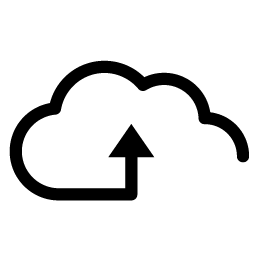
\includegraphics[width=\textwidth]{img/deployment_black.png}
          \end{figure}
          \vspace*{-2em}
          {\Huge ?}
        }
      \end{column}
    \end{columns}

    \vspace*{-2.5em}
    \begin{columns}[b]
      \begin{column}{.3\textwidth}
        \centering
        \onslide<2->{
          \begin{figure}
            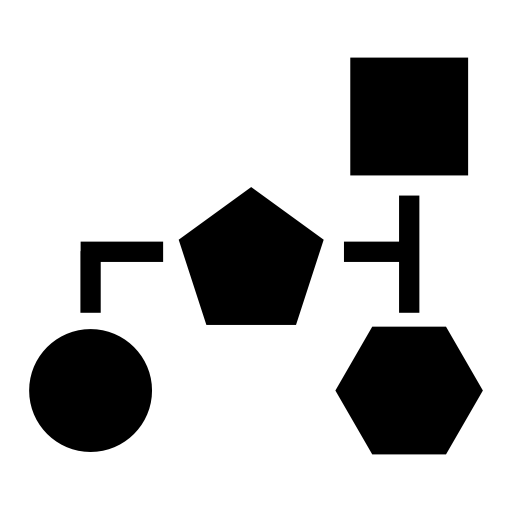
\includegraphics[width=0.7\textwidth]{img/application.png}
          \end{figure}
          {\large Application specification}
        }
      \end{column}
      \begin{column}{.3\textwidth}

      \end{column}
      \begin{column}{.3\textwidth}
        \centering
        \onslide<3->{
          \begin{figure}
            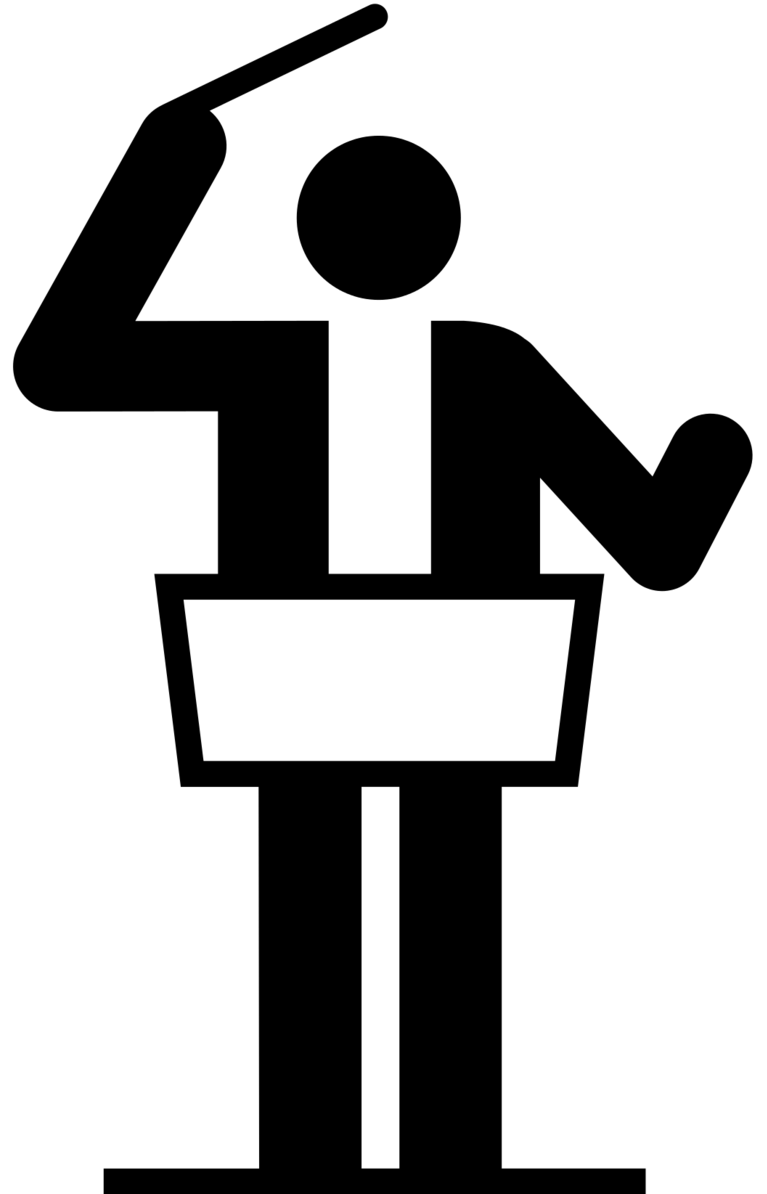
\includegraphics[width=0.6\textwidth]{img/orchestrate.png}
          \end{figure}
          {\large Application orchestration}
        }
      \end{column}
    \end{columns}

    % The execution of all the activities that make a software system available to use.
    % Nowadays strictly related to the cloud infrastructure.
    % Need of a way to express all the \textbf{requirements} that the application needs to run.
  \end{frame}


\section{Docker}\subsection*{}

  \begin{frame}{Docker}
    \begin{figure}
      
\includegraphics[width=0.5\textwidth]{img/docker.png}
    \end{figure}
    Docker is a tool that can package an application and its dependencies in a virtual container that can run on any Linux server.
    % Docker containers wrap up the software and all the requirements: code, runtime, system tools, system libraries.
    % This guarantees that the software always run in all environment that support Docker.
  \end{frame}

  \begin{frame}{VM vs Docker}
    \begin{figure}
      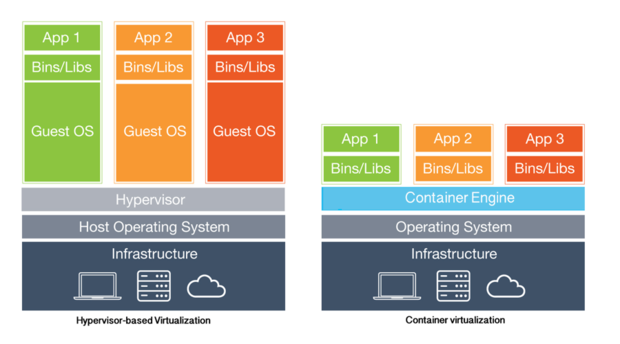
\includegraphics[width=1\textwidth]{img/docker_vs_vm.png}
    \end{figure}
  \end{frame}

  \begin{frame}{Main concepts}
    Main concepts of the Docker platform
    \begin{itemize}
      \item \textbf{Dockerfile}, a script to generate a Docker Image
      \item \textbf{Docker Image}, a separated file-system with all the binaries and library
      \item \textbf{Docker Container}, running instance of a Docker Image
      \item \textbf{Docker Volume}, a persistent data storage system
      \item \textbf{Docker Hub}, a public database of Docker Images
    \end{itemize}
  \end{frame}

  \begin{frame}{Architecture of Docker}
    \begin{figure}
      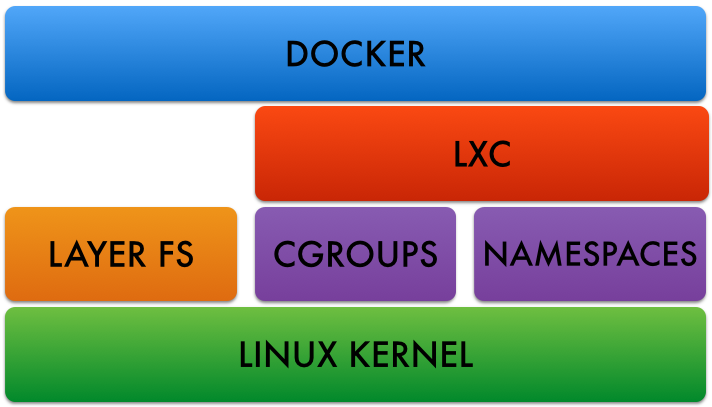
\includegraphics[width=.7\textwidth]{img/docker_achitecture_crop.png}
    \end{figure}
    \begin{itemize}
      \item \textbf{LXC}, an operating-system-level virtualization method
      \item \textbf{Layer file-system}, a Union file system
    \end{itemize}
  \end{frame}

  \begin{frame}{Layer file-system}
    \only<1>{
      Each layer is only a set of differences from the layer before it.
      \begin{figure}
        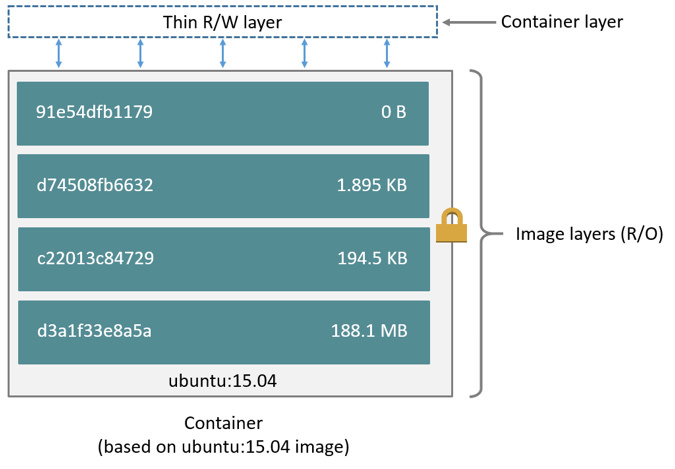
\includegraphics[width=1\textwidth]{img/container-layers.jpg}
      \end{figure}
    }
    \only<2>{
      Copy-on-write permits to share the same layer between more containers.
      \begin{figure}
        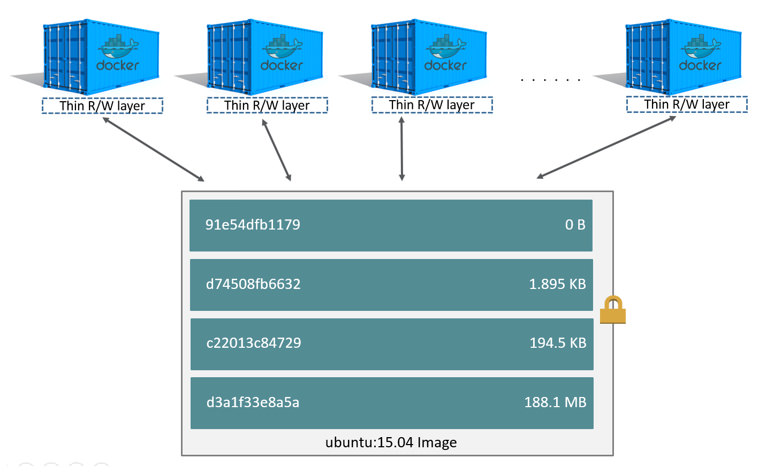
\includegraphics[width=1\textwidth]{img/sharing-layers.jpg}
      \end{figure}
    }
  \end{frame}

  \begin{frame}{How use Docker}
    \begin{figure}
      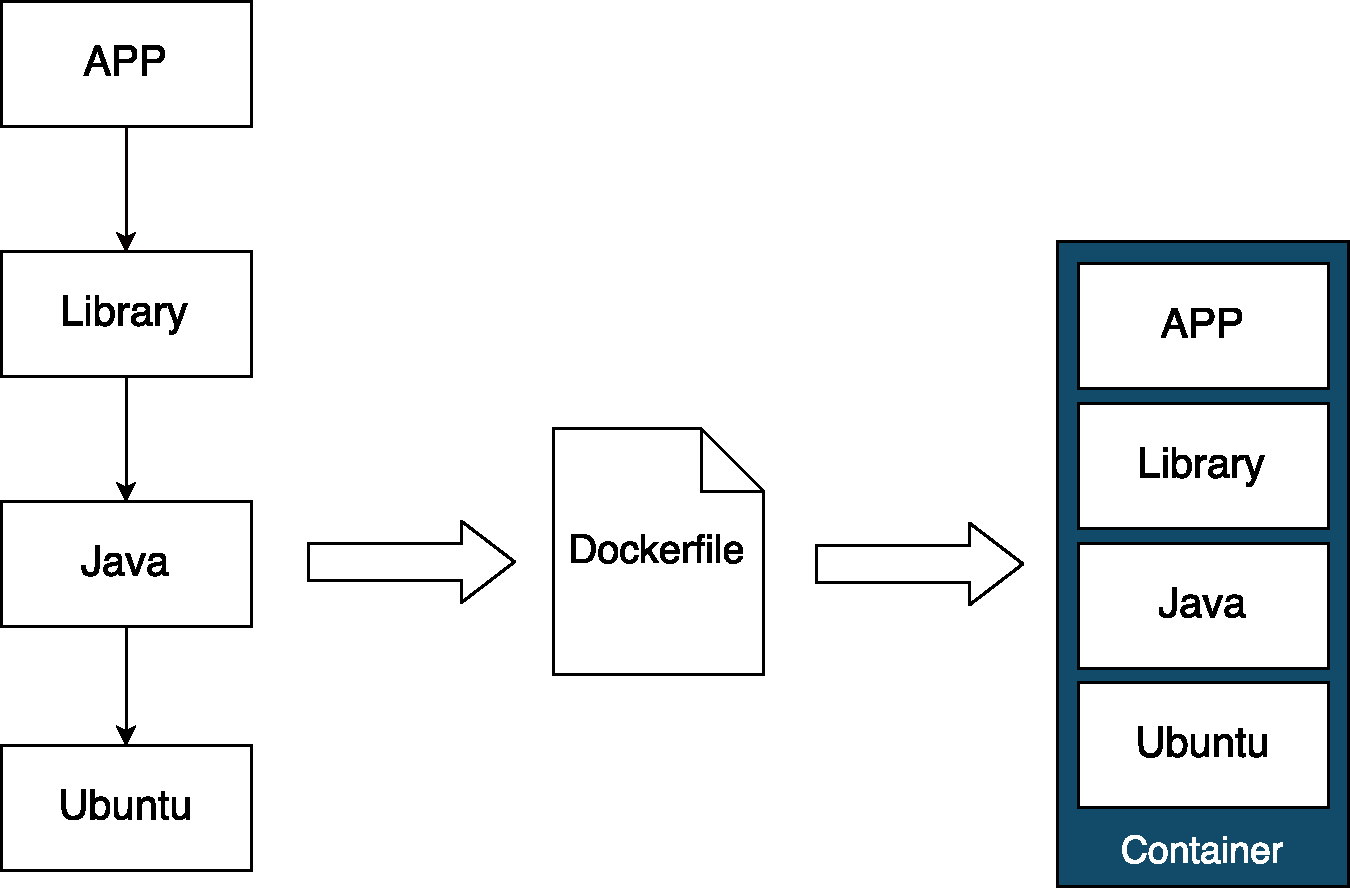
\includegraphics[width=1\textwidth]{img/docker_build.pdf}
    \end{figure}
  \end{frame}

  \begin{frame}{Multi-container application}
    \begin{figure}
      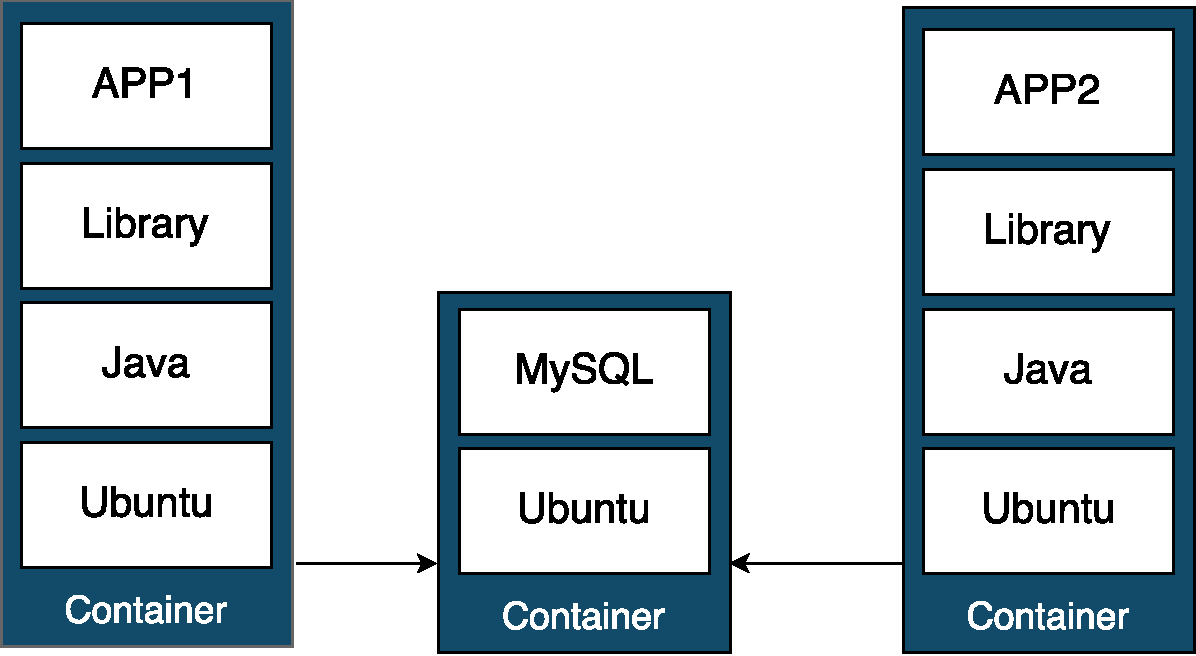
\includegraphics[width=1\textwidth]{img/docker_multicontainer.pdf}
    \end{figure}
  \end{frame}

  \begin{frame}[fragile]{Docker Compose}
    \begin{columns}[c]
      \begin{column}{.4\textwidth}
        \begin{figure}
          
\includegraphics[width=1\textwidth]{img/docker_compose.png}
        \end{figure}
      \end{column}
      \begin{column}{.6\textwidth}
      \begin{lstlisting}[basicstyle=\ttfamily,keywordstyle=\color{red}]
  version: "2"
  services:
    web:
      build: .
      ports:
       - "5000:5000"
      volumes:
       - .:/code
    redis:
      image: "redis:alpine"
      \end{lstlisting}
      \end{column}
    \end{columns}
  \end{frame}

  \begin{frame}{Problems}
    \begin{itemize}
      \item[\textcolor{red}{\textbf{--}}]<1-> The container hide the components that it contains
      \item[\textcolor{red}{\textbf{--}}]<2-> Poor application orchestration
      \item[\textcolor{red}{\textbf{--}}]<3->
      Docker containers as "minimal orchestration entities"
      %Can orchestrate only container (Docker compose)
    \end{itemize}
  \end{frame}

\section{TOSCA}\subsection*{}
  \begin{frame}{TOSCA}
    \begin{figure}
      
\includegraphics[width=0.9\textwidth]{img/oasis.png}
    \end{figure}
    OASIS standard meta-language to describe the topology of an application, with its components and relationships.
  \end{frame}

  \begin{frame}{Main concepts}
      \begin{itemize}
        \item YAML-based description
        \item CSAR archive containing TOSCA specs and executable artifacts
        \item Declarative processing
      \end{itemize}
  \end{frame}

  \begin{frame}{TOSCA description}
    \begin{figure}
      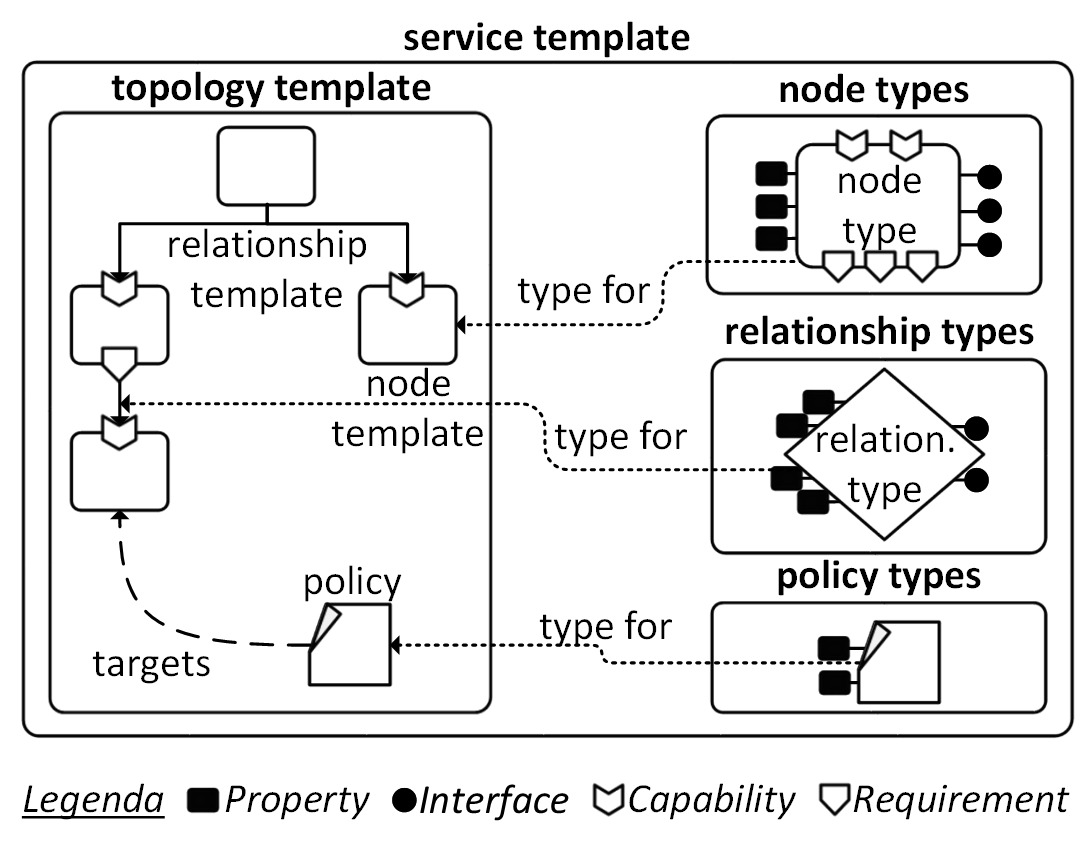
\includegraphics[width=0.9\textwidth]{img/service-template.png}
    \end{figure}
  \end{frame}

  \begin{frame}{Node type}
    \begin{figure}
      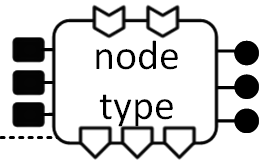
\includegraphics[width=0.3\textwidth]{img/tosca_node_type.png}
    \end{figure}
    \begin{itemize}
      \item \textbf{requirements}, what a component requires
      \item \textbf{capabilities}, what a component offers
      \item \textbf{properties}, descriptive information about a component
      \item \textbf{interfaces}, operations to deploy and manage a component
      \item \textbf{artifacts}, installables/executables/data implementing interface operations
    \end{itemize}
  \end{frame}

  \begin{frame}{How it works}
    \begin{figure}
      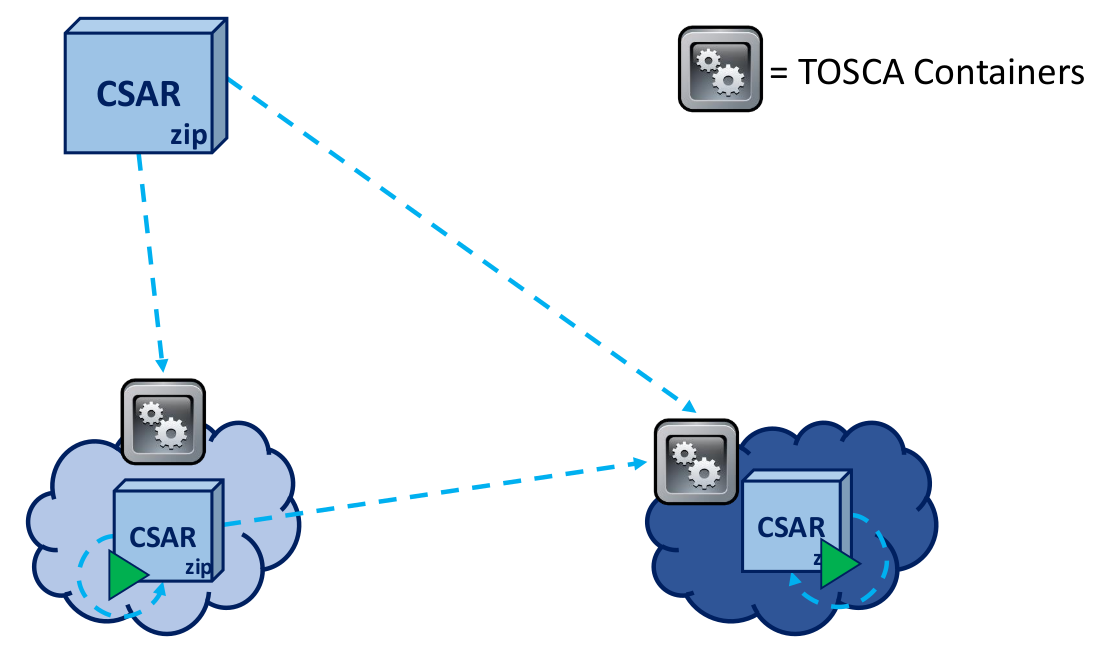
\includegraphics[width=\textwidth]{img/tosca_how.png}
    \end{figure}
    % \begin{enumerate}
    %   \item create an archive (.CSAR) whit the description and artifacts of the multi-component application
    %   \item send to an infrastructure which can process TOSCA
    %   \item following the description and using the artifacts the application can be deploy
    % \end{enumerate}
  \end{frame}

  \begin{frame}{Declarative processing - A possible execution}
    \begin{columns}[c]
      \begin{column}{.65\textwidth}
        \begin{figure}
          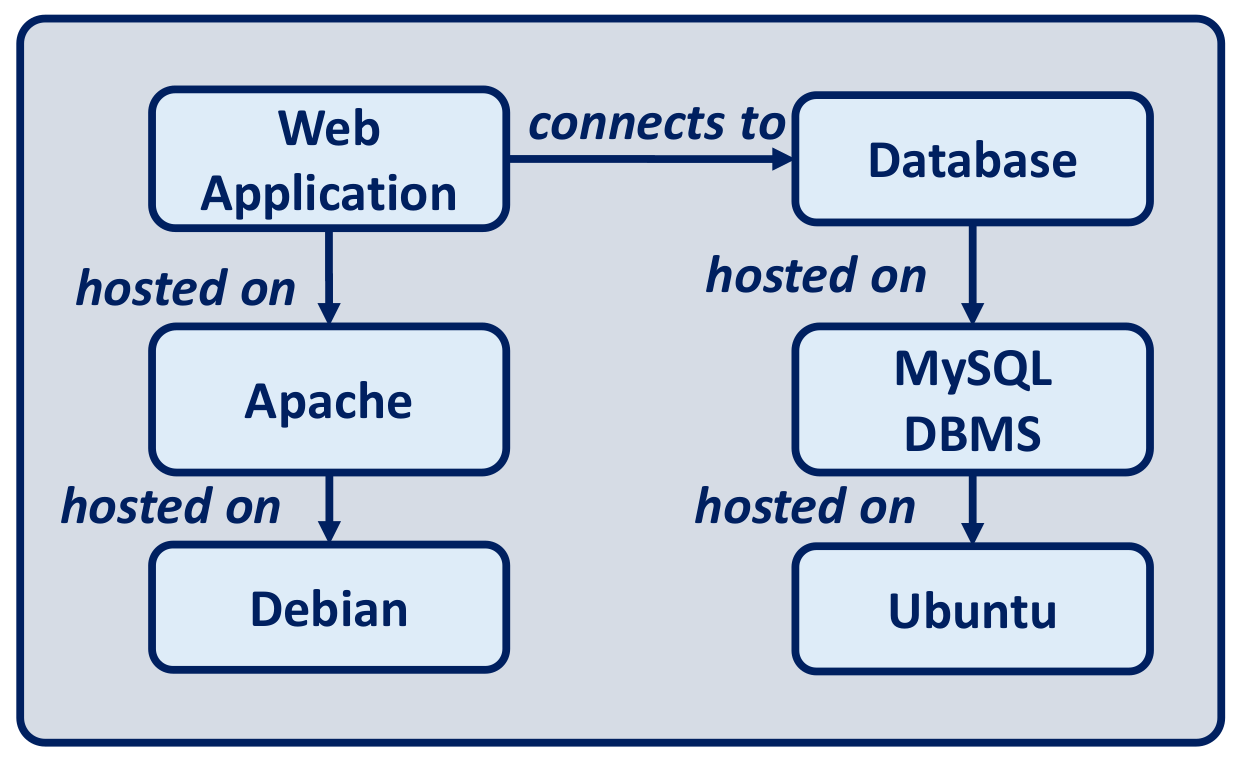
\includegraphics[width=\textwidth]{img/tosca_deploy.png}
        \end{figure}
      \end{column}
      \begin{column}{.35\textwidth}
        \begin{enumerate}
          \item<1-> Debian, Ubuntu
          \item<2-> Apache, MySQL
          \item<3-> Database
          \item<4> Web Application
        \end{enumerate}
      \end{column}
    \end{columns}
  \end{frame}

  \begin{frame}{Problems}
    \begin{itemize}
      \item[\textcolor{red}{\textbf{--}}] Specs may be too verbose
      \item[\textcolor{red}{\textbf{--}}] Lack of tools for supporting development of TOSCA apps
      \item[\textcolor{red}{\textbf{--}}] Lack of engines for running  TOSCA apps
    \end{itemize}
  \end{frame}

\section{TosKer}\subsection*{}
  \begin{frame}{TosKer}
    An orchestration engine capable of deploying, on top of Docker, applications described in TOSCA YAML.

    \begin{itemize}
      \item TosKer inputs a TOSCA description of a multi-component application, and
      \item it automatically deploys and orchestrates such application on top of the Docker engine
    \end{itemize}
  \end{frame}

  \begin{frame}{Describing applications with TosKer}
    \begin{itemize}
      \item Applications are specified as a composition of the following components:\begin{itemize}
          \item \small\emph{Docker containers} {\footnotesize\texttt{tosker.nodes.Container}}
          \item \small\emph{Docker volumes} {\footnotesize\texttt{tosker.nodes.Volume}}
          \item \small\emph{Software} {\footnotesize\texttt{tosker.nodes.Software}}
        \end{itemize}\pause
      \item Components can be interconnected with the following relationships:
      \begin{itemize}
          \item \small\emph{hosted on} {(\footnotesize\texttt{tosca.relationships.HostedOn})}
          \item \small\emph{connected to} {(\footnotesize\texttt{tosca.relationships.ConnectsTo})}
          \item \small\emph{attached to} {(\footnotesize\texttt{tosca.relationships.AttachesTo})}
          \item \small\emph{depending on} {(\footnotesize\texttt{tosca.relationships.DependsOn})}
        \end{itemize}
    \end{itemize}
  \end{frame}

  \begin{frame}{tosker.nodes.Container}
    \begin{figure}
      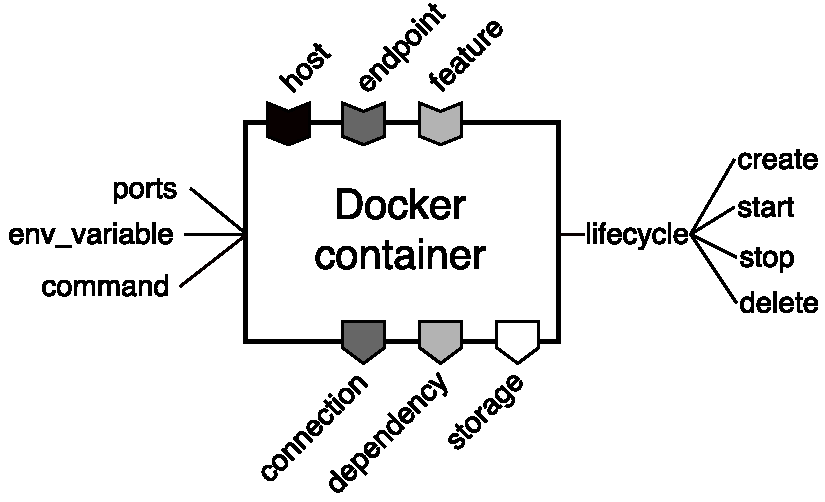
\includegraphics[width=0.8\textwidth]{img/tosker_types_container.pdf}
    \end{figure}
  \end{frame}

  \begin{frame}{tosker.nodes.Software}
    \begin{figure}
      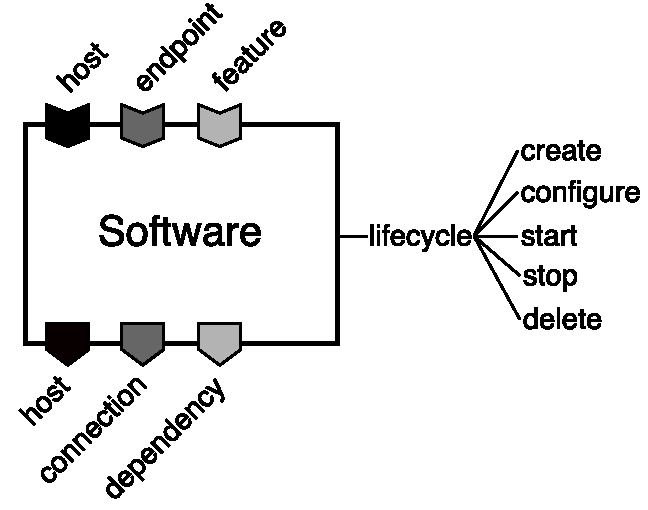
\includegraphics[width=0.8\textwidth]{img/tosker_types_software.pdf}
    \end{figure}
  \end{frame}

  \begin{frame}{tosker.nodes.Volume}
    \begin{figure}
      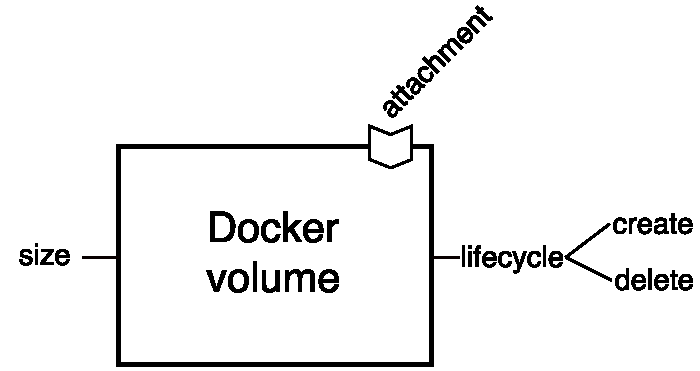
\includegraphics[width=0.8\textwidth]{img/tosker_types_volume.pdf}
    \end{figure}
  \end{frame}

  \begin{frame}{Topology constraints}
    Each application topology must satisfy a set of constraints on how to compose nodes and relationships, e.g.,
    \begin{itemize}
      \item \small A \emph{software} must be ``\emph{hosted on}'' another \emph{software} or a \emph{Docker container}
      \item \small A \emph{Docker container} and \emph{Docker volume} cannot be ``\emph{hosted on}'' other components
      \item \small Only \emph{Docker containers} can be ``\emph{attached to}'' \emph{Docker volumes}
    \end{itemize}
  \end{frame}

  \begin{frame}{Case study: Thoughts}
    \begin{figure}
      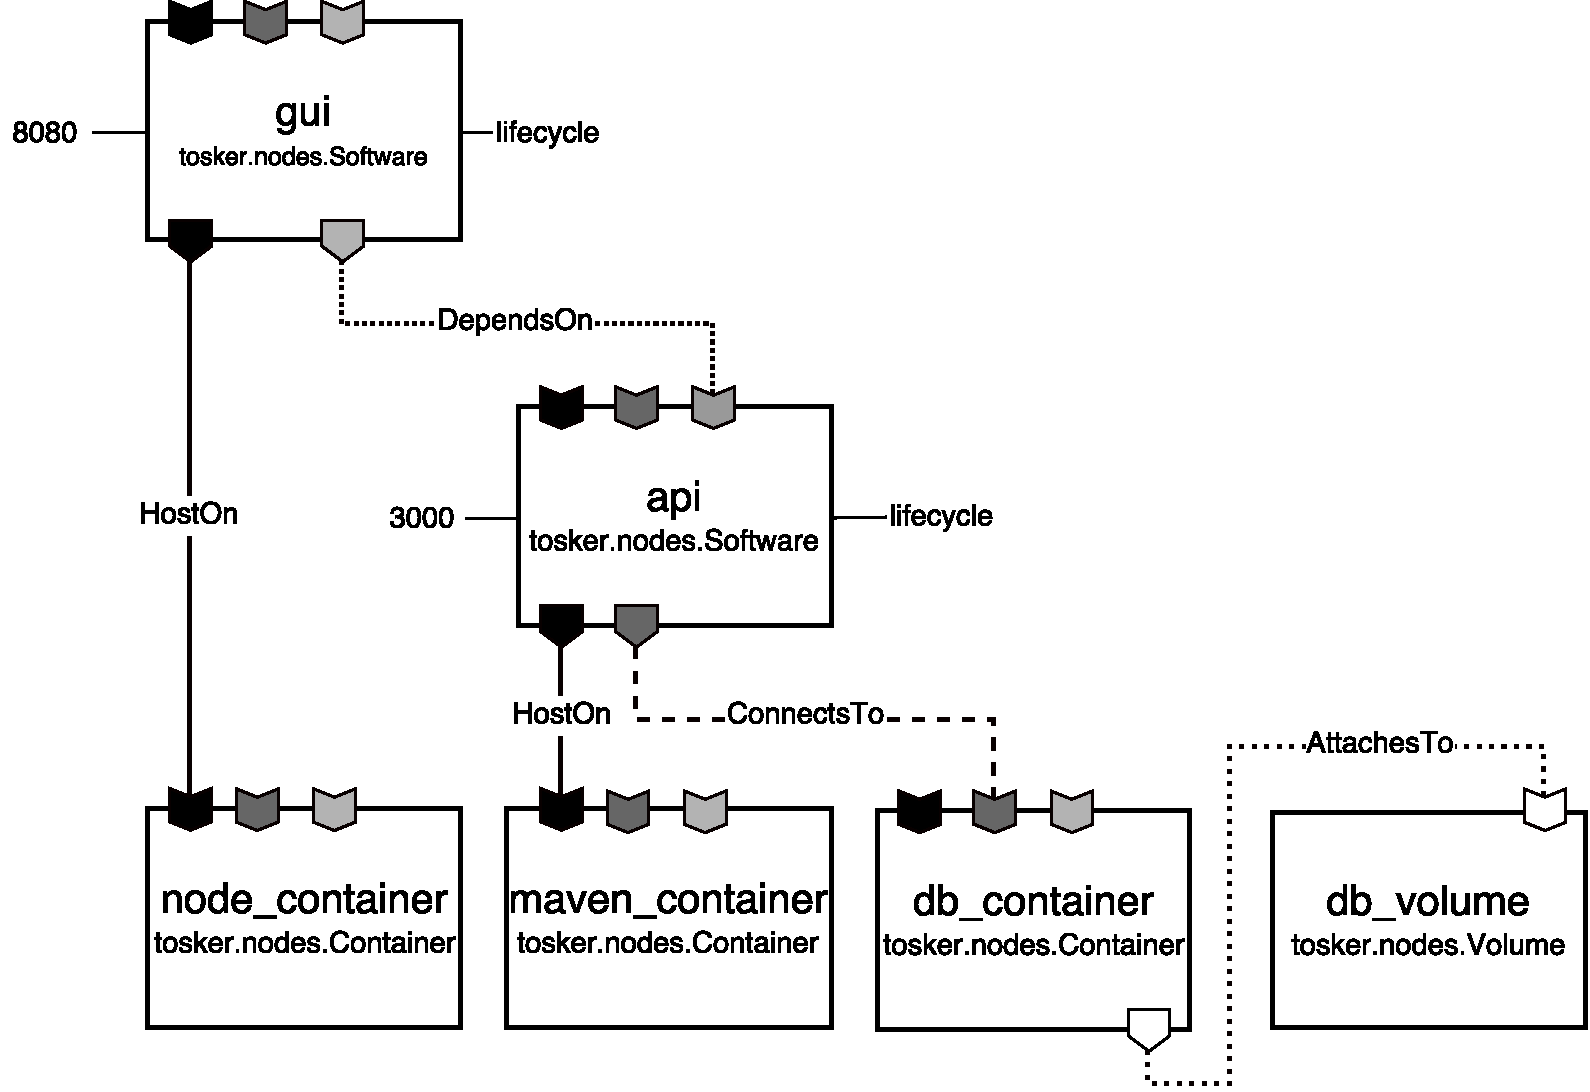
\includegraphics[width=\textwidth]{img/thoughts_architecture.pdf}
    \end{figure}
  \end{frame}

  \begin{frame}{Architecture}
    \begin{figure}
      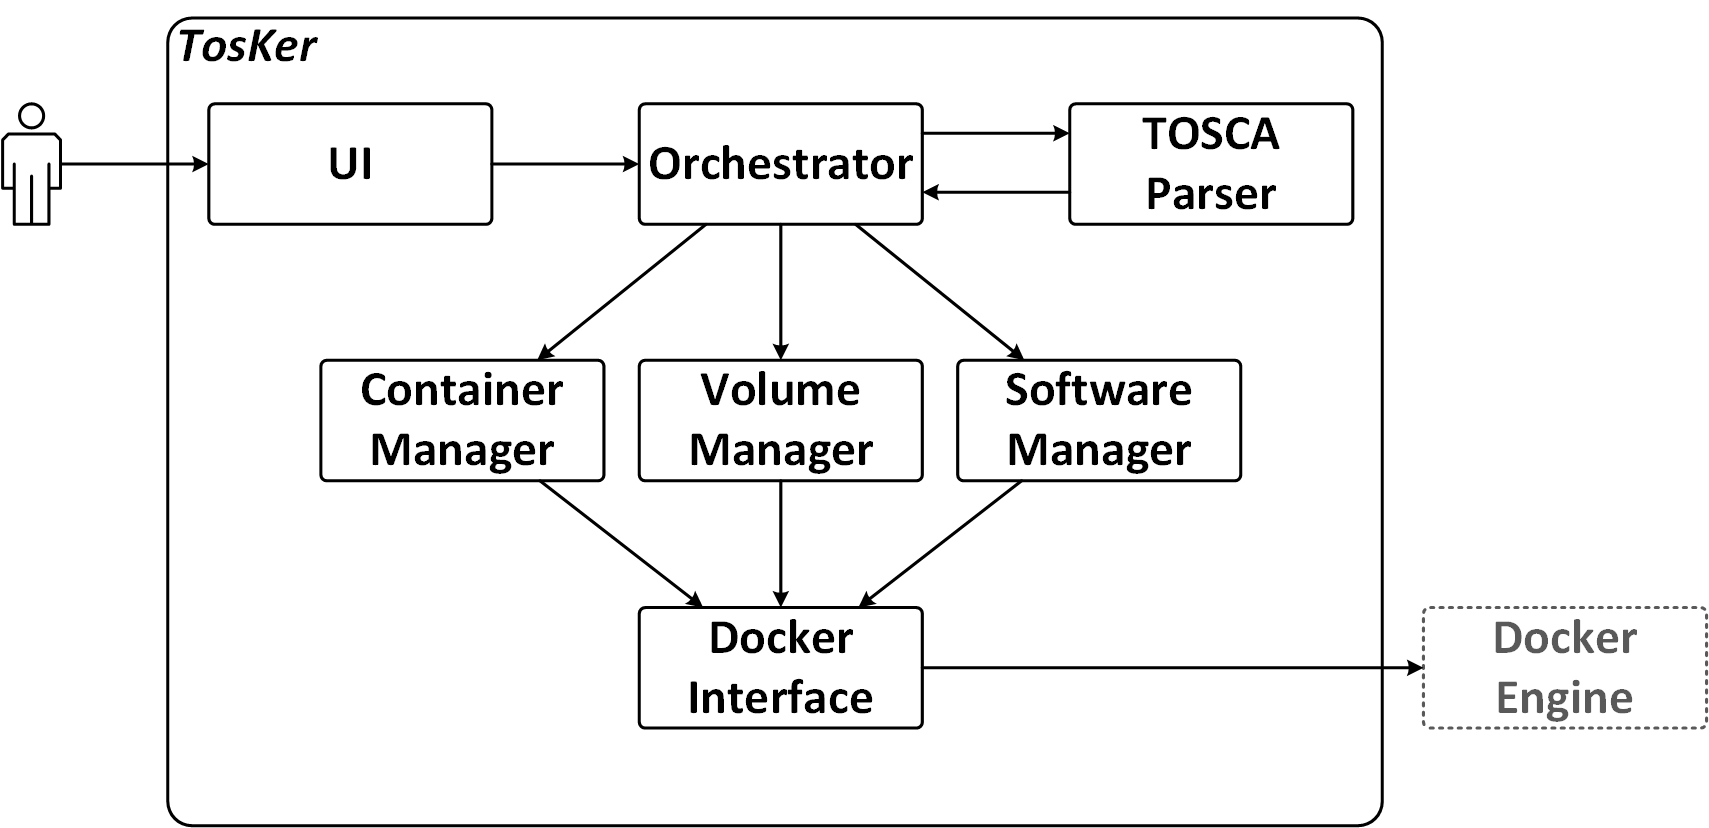
\includegraphics[width=\textwidth]{img/architecture.png}
    \end{figure}
  \end{frame}

  \begin{frame}[t]{How TosKer orchestrates applications}
    % \vspace*{-.5em}
    \only<1>{
      \begin{figure}
        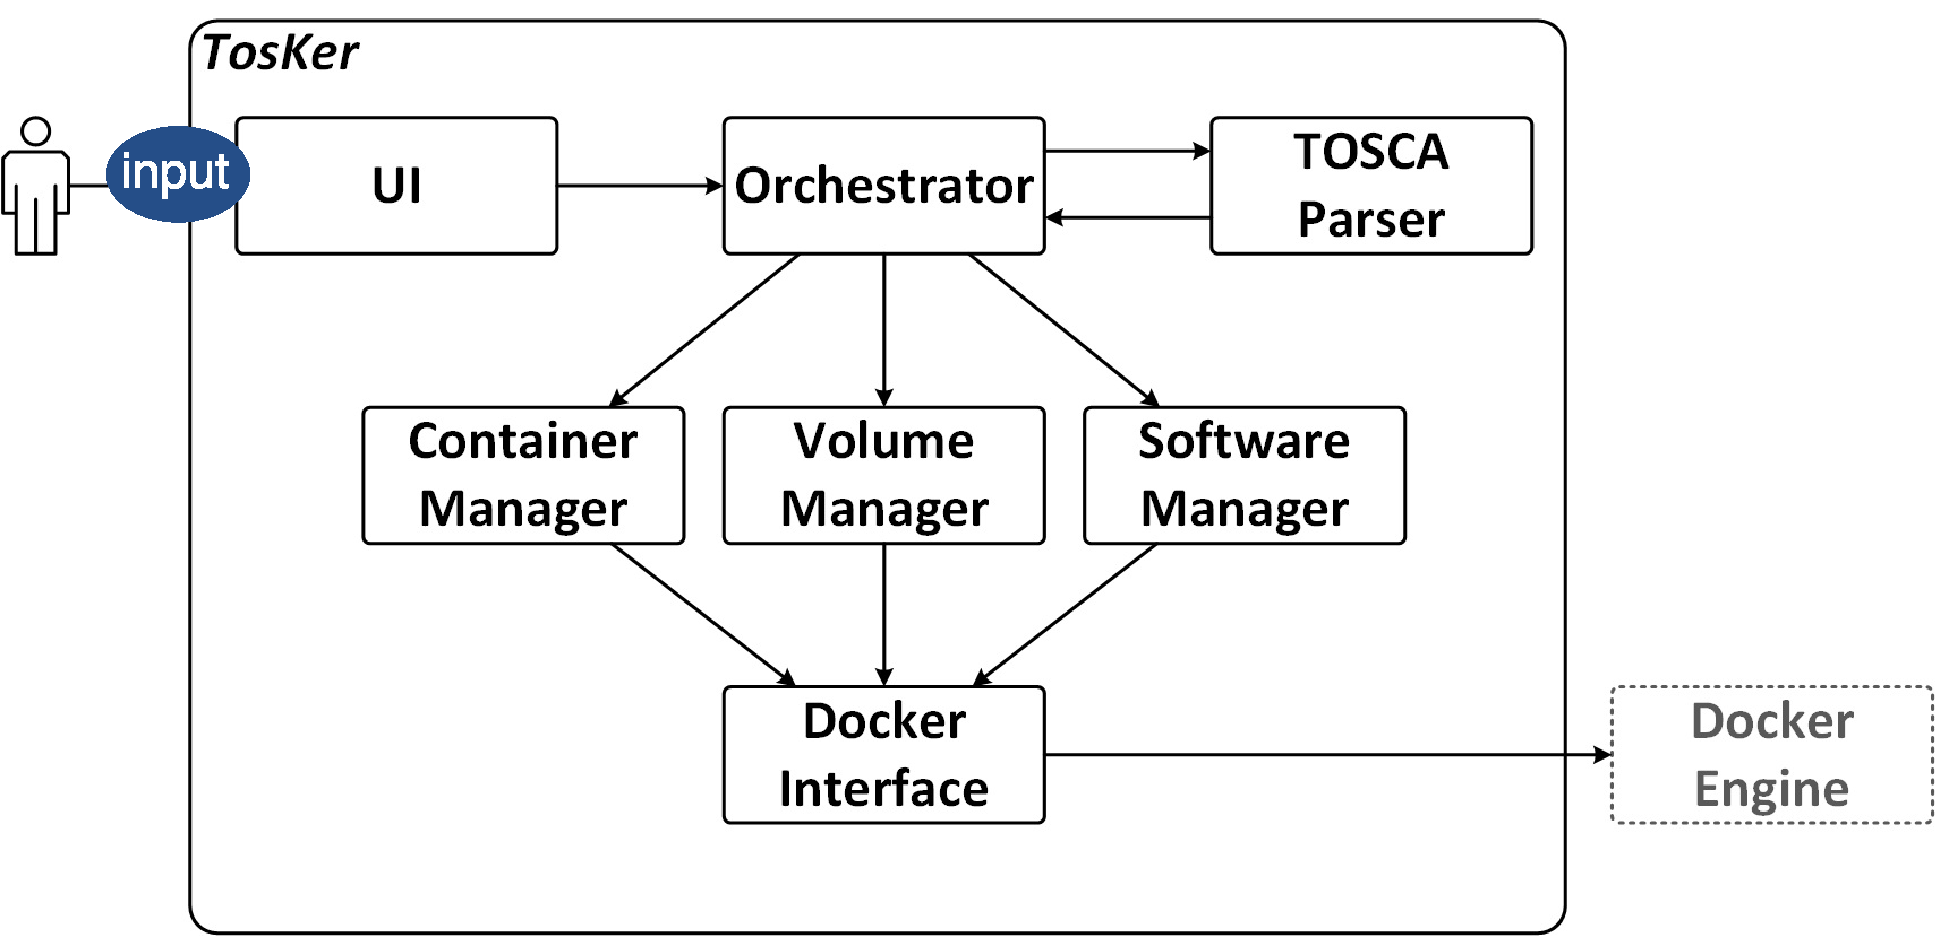
\includegraphics[width=.9\textwidth]{img/tosker_how_1.pdf}
      \end{figure}
      The input of TosKer is
      \begin{itemize}
        \item a TOSCA application specified using TosKer types, and
        \item management operation(s) to perform.
      \end{itemize}
    }
    \only<2>{
      \begin{figure}
        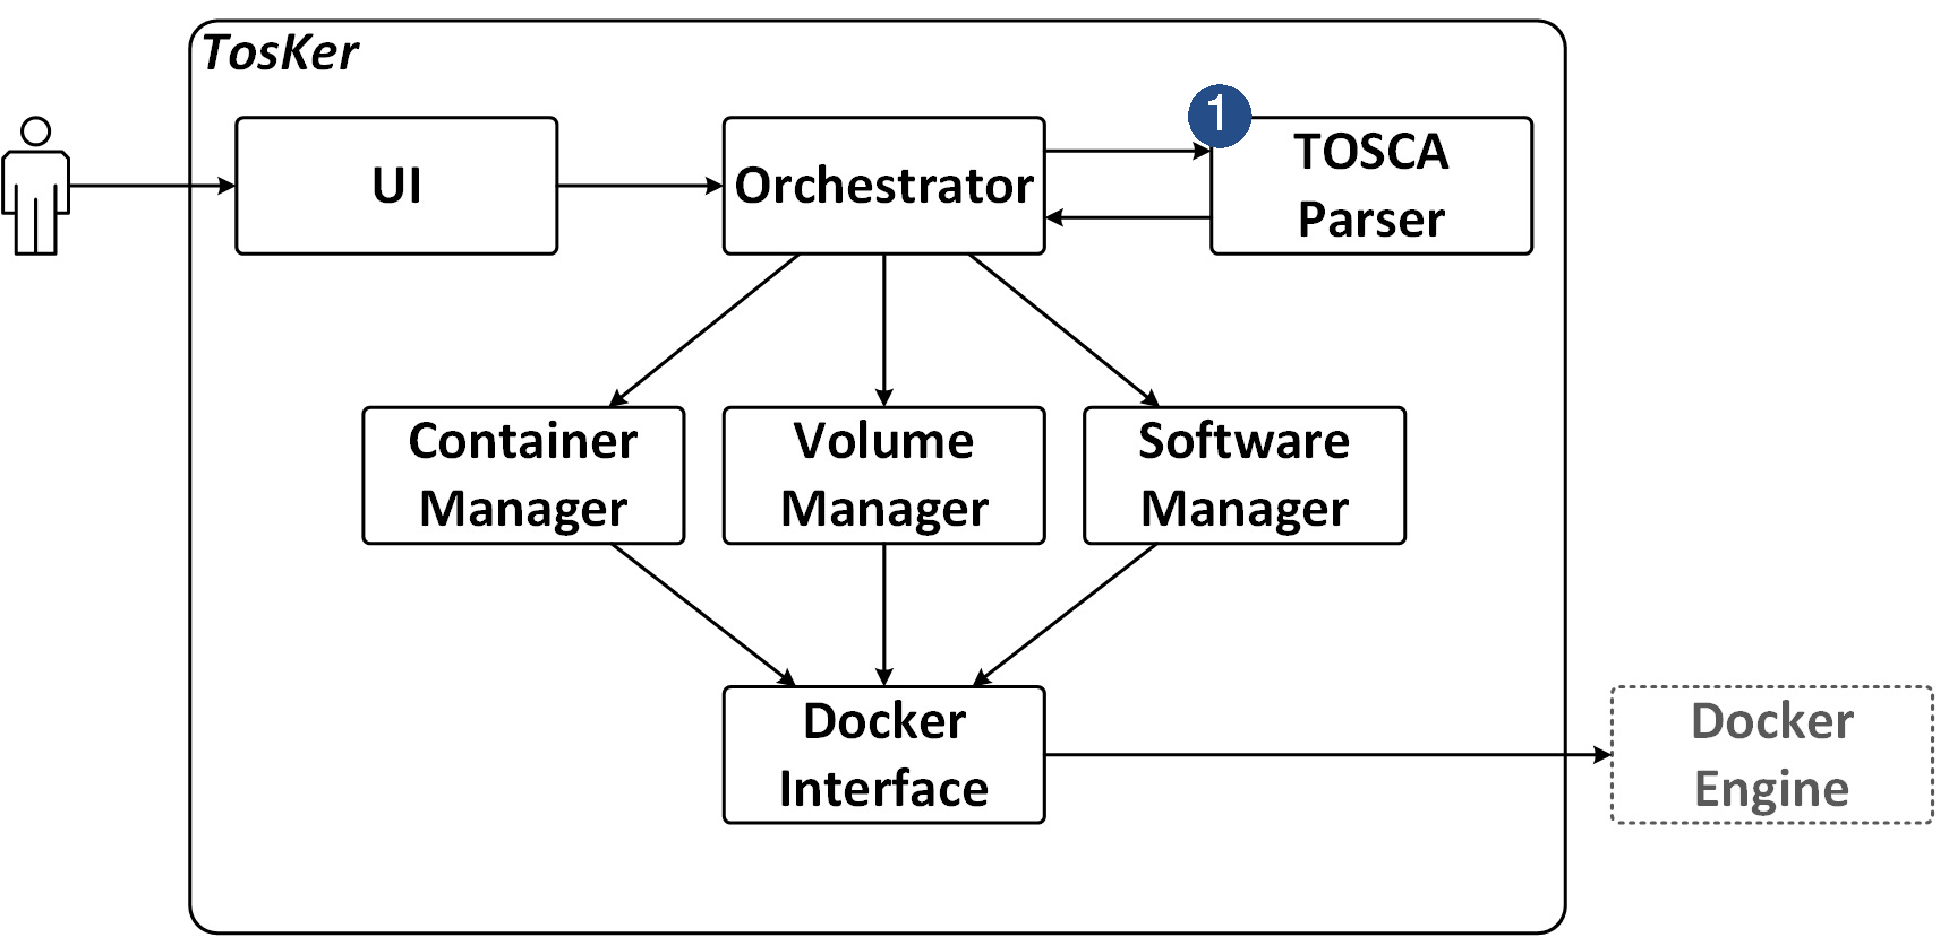
\includegraphics[width=.9\textwidth]{img/tosker_how_2.pdf}
      \end{figure}
      \vspace*{-.5em}
      TosKer
      \begin{itemize}
        \item parses and validates the TOSCA application, and
        % \item create an internal representation of the application
        \item executes a topological sorting algorithm.
      \end{itemize}
    }
    \only<3>{
      \begin{figure}
        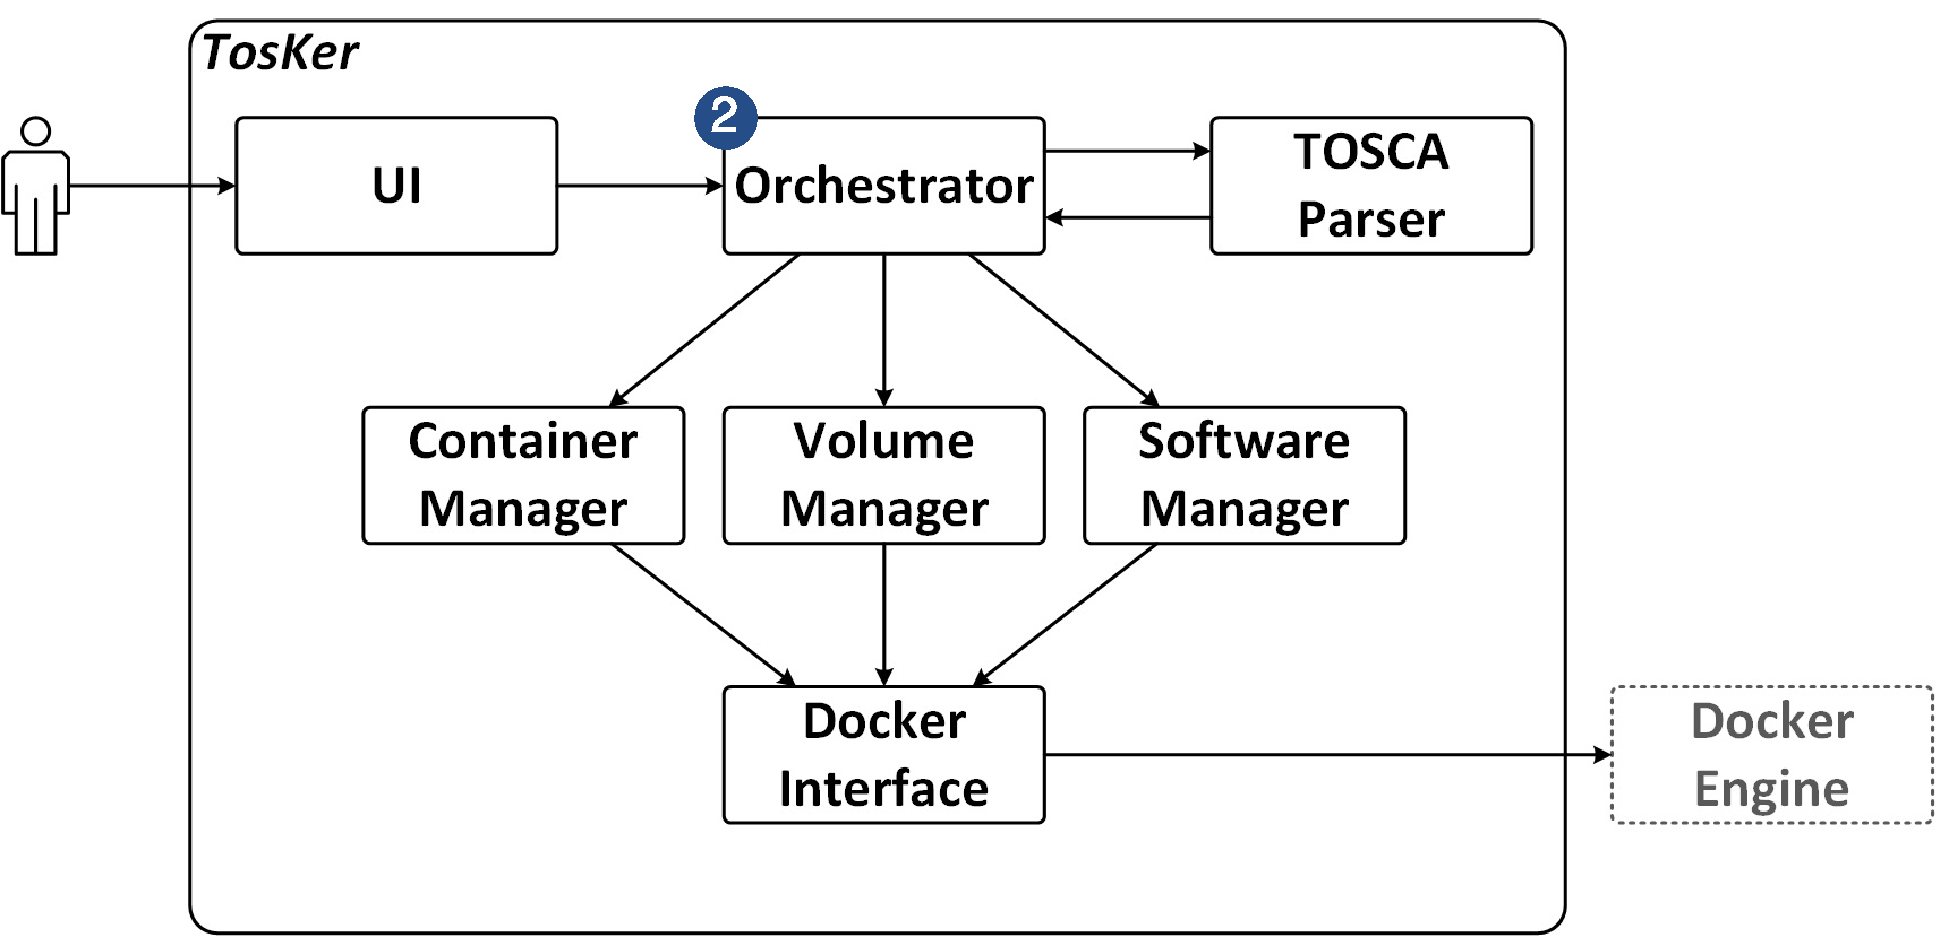
\includegraphics[width=.9\textwidth]{img/tosker_how_3.pdf}
      \end{figure}
      \vspace*{-.5em}
      TosKer %exploits the (topologically sorted) application to orchestrate it:
      \begin{itemize}
        \item scans the sorted application topology, and
        \item for each component, it calls a specific operation (e.g., create)
      \end{itemize}
    }
    \only<4>{
      \begin{figure}
        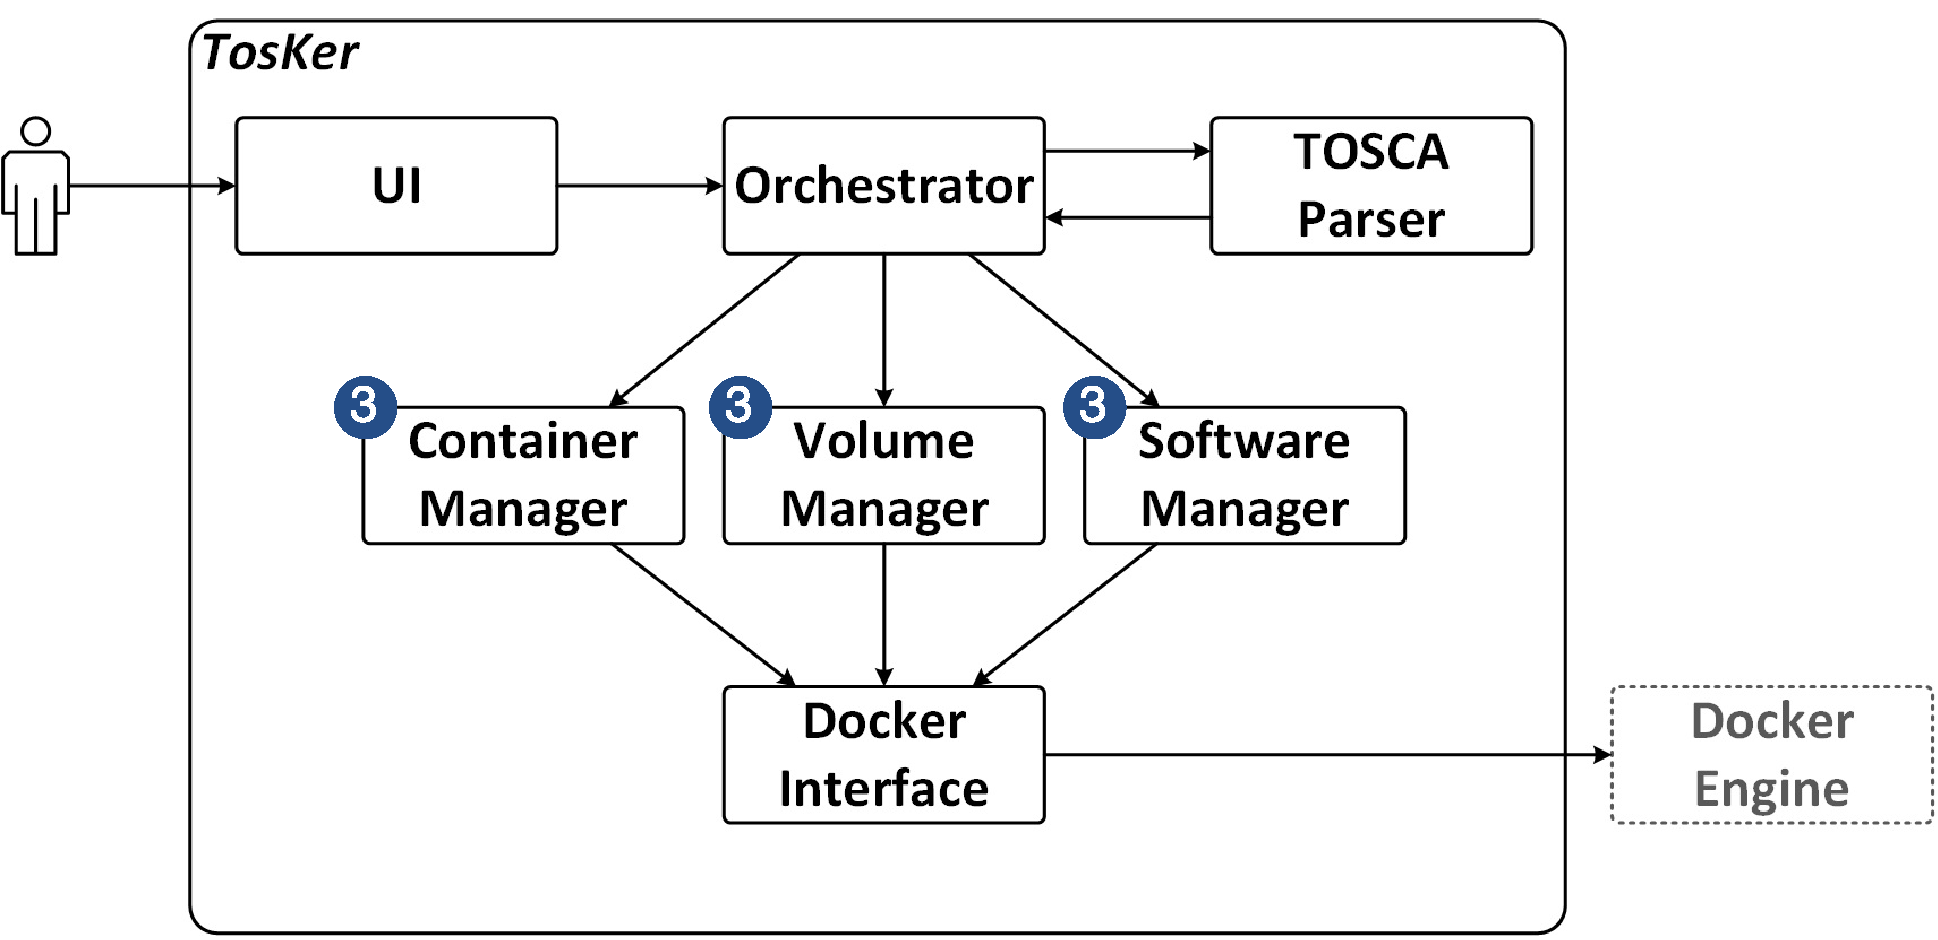
\includegraphics[width=.9\textwidth]{img/tosker_how_4.pdf}
      \end{figure}
      Each manager is in charge of implementing/executing the invoked operation on a component...
    }
    \only<5>{
      \begin{figure}
        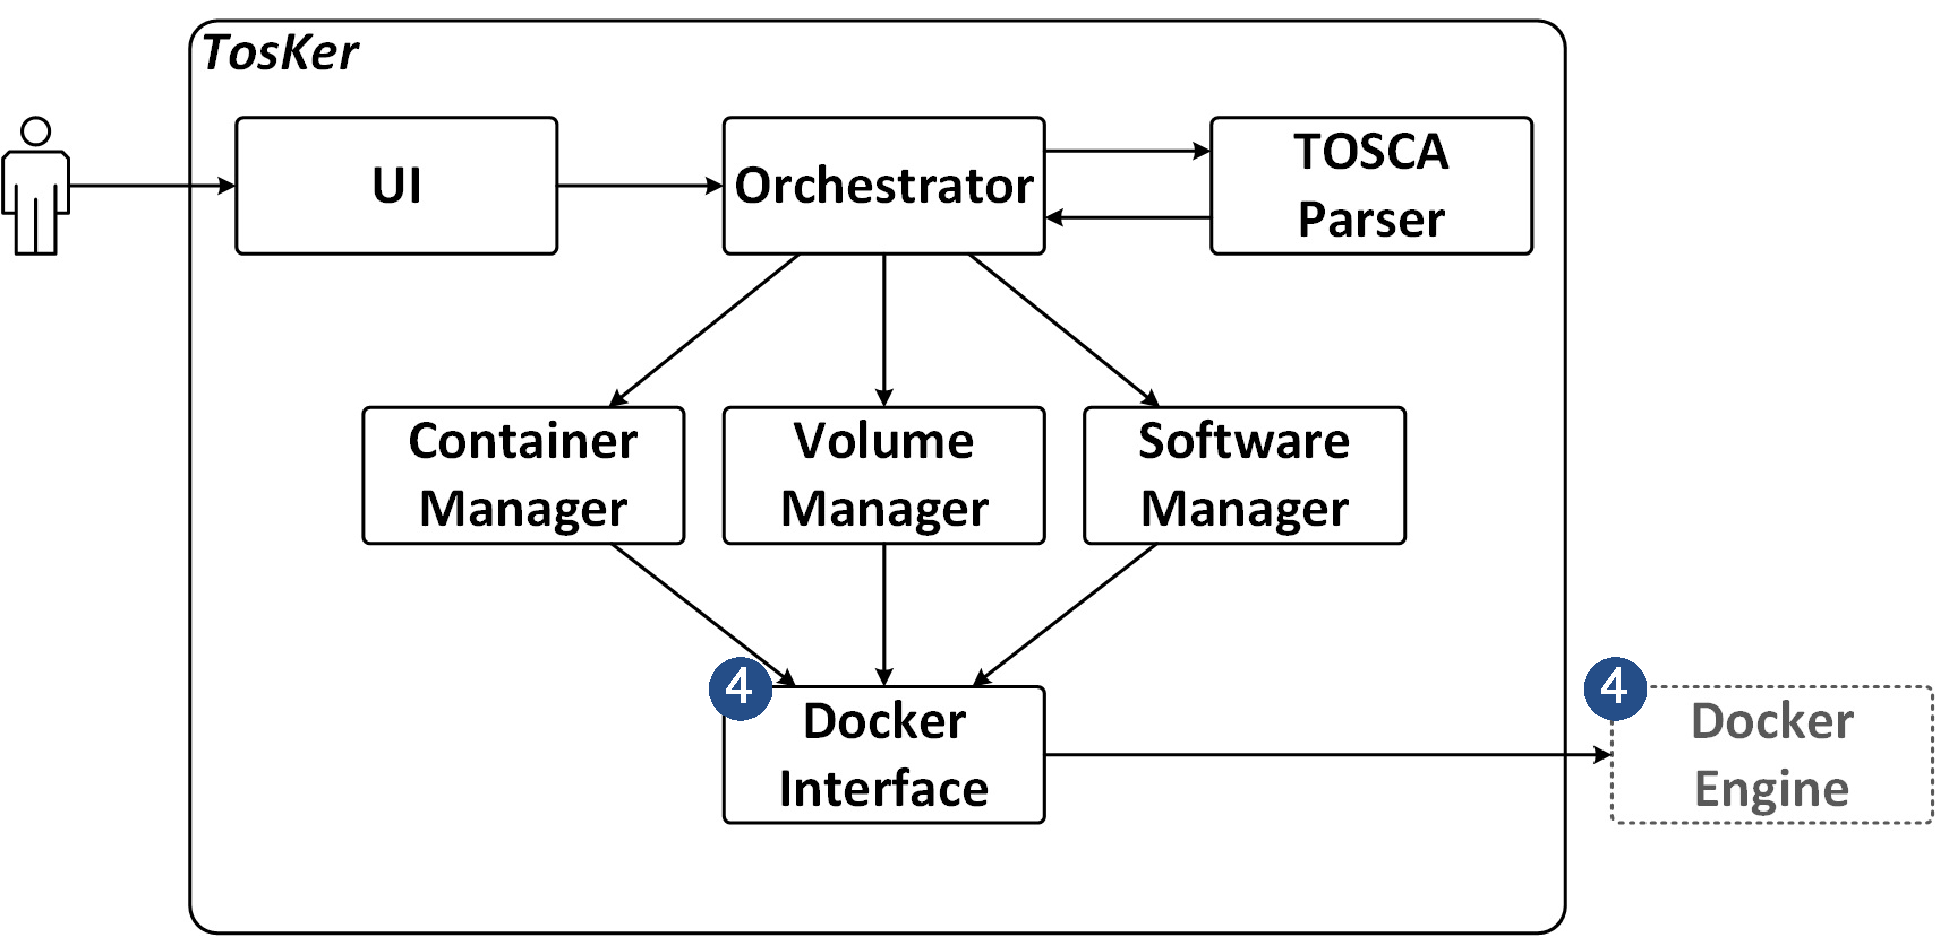
\includegraphics[width=.9\textwidth]{img/tosker_how_5.pdf}
      \end{figure}
      ...by properly invoking the Docker engine (through the Docker interface)
    }
  \end{frame}

  \begin{frame}{Implementation}
    \begin{columns}[b]
      \begin{column}{.3\textwidth}
        \centering
        % \onslide<1->{
          \begin{figure}
            
\includegraphics[width=.6\textwidth]{img/python.png}
          \end{figure}
          {\large Python}
        % }
      \end{column}
      \begin{column}{.3\textwidth}
        \centering
        % \onslide<2->{
          \begin{figure}
            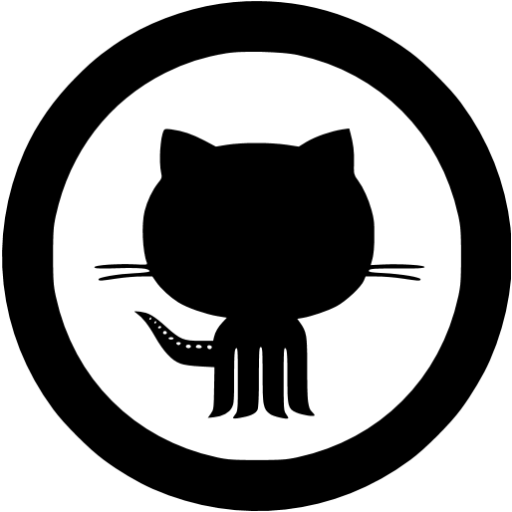
\includegraphics[width=.6\textwidth]{img/github.png}
          \end{figure}
          {\large GitHub}
        % }
      \end{column}
      \begin{column}{.3\textwidth}
        \centering
        % \onslide<2>{
          \begin{figure}
            
\includegraphics[width=.6\textwidth]{img/mit.png}
          \end{figure}
          {\large MIT Licence}
        % }
      \end{column}
    \end{columns}
      \vspace{20pt}
      \begin{itemize}
        \item %\onslide<1->{
          \small\textbf{PyPI}: \href{https://pypi.python.org/pypi/tosKer}{https://pypi.python.org/pypi/tosKer}\\
          \indent\indent\texttt{pip install tosker}\vspace{10pt}
        % }
        \item %\onslide<2>{
          \small\textbf{GitHub}: \href{https://github.com/di-unipi-socc/TosKer}{https://github.com/di-unipi-socc/TosKer}
        % }
      \end{itemize}
  \end{frame}

\section{Conclusions and Future work}\subsection*{}
  \begin{frame}{Conclusions}
    %The objective of this thesis was to design and prototype \dt an orchestration engine, which
    \onslide<1->{
    We focussed on the problem of orchestrating the deployment and management of composite cloud applications.
    \begin{itemize}
      \item Docker
      \item TOSCA YAML
    \end{itemize}
    }
    \bigskip
    \onslide<2>{
    We presented the TosKer orchestration engine, which
    \begin{itemize}
      \item extends TOSCA by providing a Docker-based orchestration engine for TOSCA applications, and
      \item extends Docker by adding the capability of orchestrating software components together with Docker containers/volumes
    \end{itemize}
    }
    % \begin{itemize}
    %   \item Approach the problem of automatically deploying and managing of applications\pause
    %   \item Study a solution to exploit the advantages of TOSCA and Docker\pause
    %   \item Design and prototype \dt, the first orchestrator engine that manage software components and Docker components together.\pause
    % \end{itemize}
  \end{frame}

  \begin{frame}{Future work}
    \begin{itemize}
      \item Automatically determine the Docker containers needed to effectively run an application (\textbf{Dockerizer})
      \item Support cluster of workstations and external cloud services
      \item Integrate TosKer with fault-aware management protocols
    \end{itemize}
  \end{frame}

  \begin{frame}{Focus on \textbf{Dockerizer}}
    \onslide<1->{
    \textbf{Dockerizer}, a completer of TosKer specifications.
    }
    \onslide<2>{
      \begin{figure}
        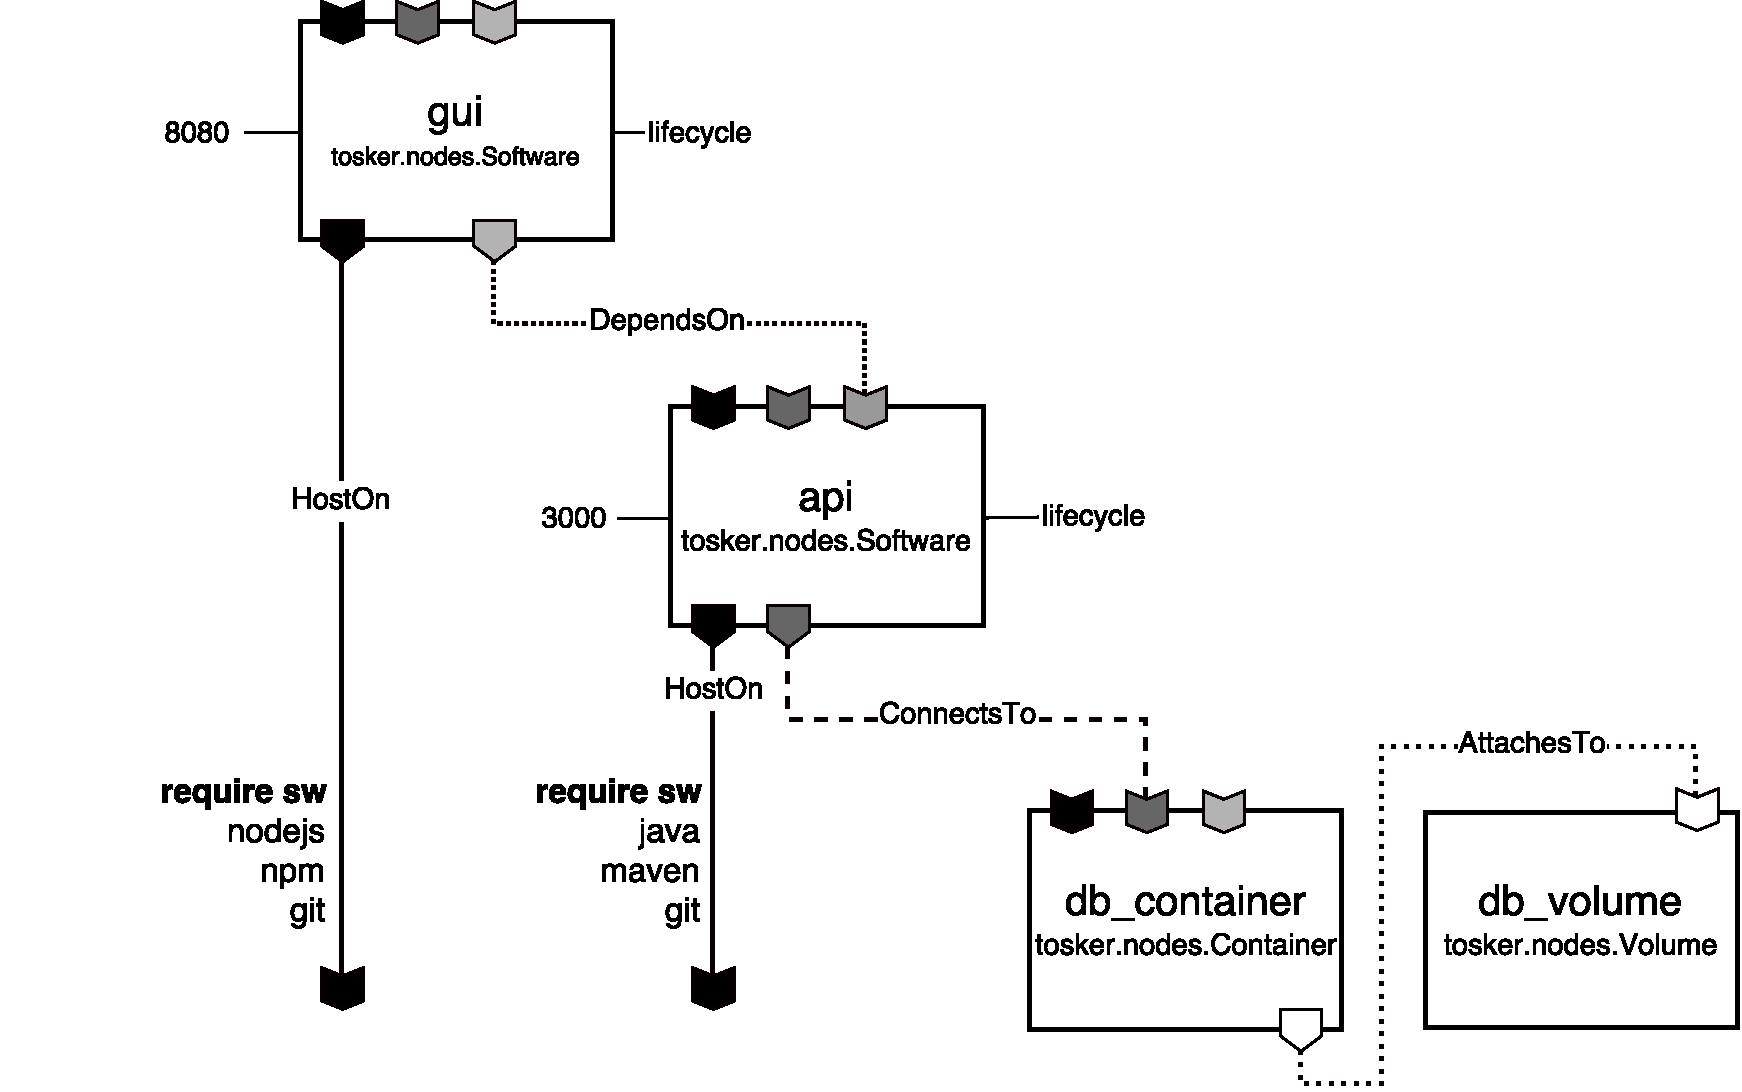
\includegraphics[width=\textwidth]{img/dockerize_example.pdf}
      \end{figure}
    }
  \end{frame}

  \begin{frame}
    \centering
    \Huge Thank You \\
    \bigskip
    \LARGE Q\&A
  \end{frame}
\end{document}
